% PROGRAMA DE PÓS-GRADUAÇÃO EM ECONOMIA APLICADA
% UNIVERSIDADE FEDERAL DO RIO GRANDE - FURG

% ===========================================================

\documentclass[a4paper, 11pt]{article}

%%%%%%%%%%%%%%%%%%%%%%%%% PACOTES %%%%%%%%%%%%%%%%%%%%%%%%%%%%%%%%%%

\usepackage[margin = 0.5in, bottom = 2in]{geometry}
\usepackage[utf8]{inputenc}
\usepackage[T1]{fontenc}
\usepackage{graphicx} 
\usepackage{xcolor}
\usepackage{lipsum}	
\usepackage{amsfonts,amsmath,amssymb, amsthm} 
\usepackage{booktabs}
\usepackage{hyperref}  
\usepackage{yhmath} 
\usepackage{tikz}

% Configuração da Fonte
\usepackage{times} % Fonte: Times New Roman

% PACOTES ESSENCIAIS
\usepackage{caption}
\usepackage{subcaption}  

%\setlength{\footskip}{0pt} % Espacio entre texto y pie de página
\renewcommand{\footnoterule}{\vspace{5pt}\hrule width 0.3\linewidth\vspace{5pt}}
\setlength{\textheight}{770pt}
\setlength{\headsep}{10pt}
\setlength{\topmargin}{-60pt}

\begin{document} %Início do Documento

%\layout
%\newpage 
\- \vspace{-0.3in}
\par\noindent\includegraphics[width = \textwidth]{Imagens/Header.png} 

%%%%%%%%%%%%%%%%%%%%%%%% CONFIG. DO TÍTULO %%%%%%%%%%%%%%%%%%%%%%%%
%\vspace{-1.8in}

\begin{center} %Inicia a centralização
\textbf{Topología | 2025-I}    \\ {\small 
Nestor Heli Aponte Avila\(^1\) \\ 
\href{mailto:n267452@dac.unicamp.br}{\url{n267452@dac.unicamp.br}}} %\\
%Prof. Piper Pimienta \\
%\href{mailto:pipe@dac.unicamp.br}{\url{pipe@dac.unicamp.br}}}

\end{center} %Finaliza a centralização

%%%%%%%%%%%%%%%%%%%%%%%%% PREAMBULO %%%%%%%%%%%%%%%%%%%%%%%%%%%%%%%%%%

\theoremstyle{definition}
\newtheorem*{definition}{\rotatebox{45}{\large \(\square\)}}

\theoremstyle{plain}
\newtheorem*{lemma}{{\scriptsize \(\square\)}}
\newtheorem*{proposition}{{\large \(\square\)}}
\newtheorem*{theorem}{{\large \(\blacksquare\)}}

\makeatletter
% Eliminar la puntuación del estilo 'plain' y 'definition'
\def\@thm@headpunct{} % Elimina el punto de los títulos de los teoremas

% Modificar el estilo de 'plain' y 'definition'
\def\th@plain{%
  %\thm@headfont{\normalfont\bfseries} % Mantener la fuente normal, sin negrita
  %\thm@notefont{\normalfont} % El texto de la nota (si la hay) no será en negrita
  \thm@headpunct{} % Sin puntuación adicional
}

\def\th@definition{%
  %\thm@headfont{\normalfont\bfseries} % Fuente normal para el título
  %\thm@notefont{\normalfont} % El texto de la nota (si la hay) no será en negrita
  \thm@headpunct{} % Sin puntuación adicional
}

\def\th@remark{%
  %\thm@headfont{\normalfont\bfseries} % Fuente normal para el título
  %\thm@notefont{\normalfont} % El texto de la nota (si la hay) no será en negrita
  \thm@headpunct{} % Sin puntuación adicional
}
\makeatother

\theoremstyle{remark}
\newtheorem*{example}{Ejemplo}
\newtheorem*{exercise}{Ejercicio}
\newtheorem*{note}{\(*\)}

\newcommand{\R}{\mathbb{R}}
\newcommand{\N}{\mathbb{N}}
\newcommand{\U}{\mathcal{U}}
\newcommand{\V}{\mathcal{V}}
\newcommand{\F}{\mathcal{F}}
\newcommand{\E}{\vspace{0.2in}}
\newcommand{\ab}{{\rotatebox{0}{\scriptsize$\lor$}}}
\newcommand{\ce}{{\text{\ \large \rotatebox{90}{$\triangleleft$}}}}

%%%%%%%%%%%%%%%%%%%%%%%%%% CONTENIDO %%%%%%%%%%%%%%%%%%%%%%%%%%%%%%%%

\section*{Conjuntos}

\- \hrule  
\begin{proposition}
  \textbf{Ejercicio} \emph{(Leyes de De Morgan.)} \(\displaystyle X\backslash \bigcup A_i = \bigcap X\backslash A_i\) \ \ y \ \ \(\displaystyle X \backslash\bigcap A_i = \bigcup X\backslash A_i\). 
\end{proposition}

\begin{exercise}
  La imagen inversa es bien portada, con uniones, intersecciones y complementos. 
\end{exercise}

\begin{exercise} {\small
  \((a) \ \displaystyle f\left(\bigcup A_i\right) = \bigcup f(A_i); \ (b)\  f\left(\bigcap A_i\right) \subset \bigcap f(A_i)\ \footnote{Igualdad si \(f\) inyecta.}; \ (c)\ \overset{\hookrightarrow}{f}(X \backslash A) \subset Y \backslash f(A); \ (d) \  \overset{\twoheadrightarrow}{f}(X\backslash A) \supset Y\backslash f(A) .\)  
  }
\end{exercise}

\begin{proposition}
  \textbf{Ejercicio} \(\displaystyle \ (a)\  A\subset f^{-1}(f(A))\text{ igualdad si } \overset{\hookrightarrow}{f}; \ (b) \  f(f^{-1}(B)) \subset B \text{ igualdad si } \overset{\twoheadrightarrow}{f}\). 
\end{proposition}
\hrule 

\section*{Espacios Métricos}

\begin{definition}
    \emph{Métrica.} Una función \(d:X\times X\to \mathbb{R}^+\) es métrica si \(\forall x,y,z \in X\)  
    \begin{itemize}
        \item \(d(x,y)\geq 0\) e \(d(x,y)=0\) si y solo si \(x = y\). 
        \item \(d(x,y) = d(y,x)\). 
        \item \(d(x,y) \leq d(x,z) + d(z,y)\). 
    \end{itemize}
\end{definition}

\E

\hrule 
\begin{example}
    Las métricas estándar en \(\R^n\) inducidas por las normas \(\|\cdot\|_j\) con \(j = 1, 2 \text{\ y\ }\infty\). 
\end{example}
\begin{example}
    Métrica discreta y métrica inducida. 
\end{example}
\hrule 

\E

\begin{definition}
    \emph{Bola abierta} \(\ \to B(a;r) := \{x\in X : d(x,a) < r\}\); \ \emph{Bola cerrada} \(\ \to B[a;r]:= \{x\in X : d(x,a)\leq r\}\). 
\end{definition}
\begin{definition}
   \(\U^\ab \subset X\) sii \(\forall x\in \U, \exists r>0\) tal que \(B(x;r)\subseteq \U\). En contraposición, \(\F^\ce\subset X \) sii \(X\backslash \F\) es abierto. 
\end{definition}

\E

\hrule 
\begin{exercise}
    Las bolas abiertas son abiertos y las cerradas son cerradas en \(X\). 
\end{exercise}
\hrule 

\E

\begin{proposition}
    Sea \(X\) un espacio métrico, entonces: \((a)\) \(\emptyset\text{ y } X\) son abiertos; \((b)\) Unión de una familia arbitraria de abiertos es abierto y \((c)\) Intersección de una familia finita de abiertos es abierto. 
\end{proposition} 
\begin{note}
    Colorario de esto es la contra-versión para cerrados. 
\end{note}
\begin{definition}
    \emph{Continuidad.} Sean \(X\text{\ y\ }Y\) espacios métricos. Una función \(f:X\to Y\) es continua en \(a\in X\) sii \(\forall\epsilon >0,\exists \delta >0\) tal que \(f(B(a;\delta))\subset B(f(a);\epsilon)\). 
\end{definition}
\begin{proposition}
    \(f:X\to Y\) es continua en \(a\in X\) sii \(\forall\ \overset{\overset{\text{$f(a)$}}{\rotatebox{-90}{$\in$}}}{V^\ab}\subset Y, \exists \ \overset{\overset{\text{$a$}}{\rotatebox{-90}{$\in$}}}{U^\ab}\subset X\) tal que \(f(U)\subset V\). 
\end{proposition}
\begin{proposition}
    \(f\) es continua \(\Leftrightarrow \ \forall \ V^\ab\subset Y\) tenemos \(f^{-1}(V)^\ab \subset X\) \(\Leftrightarrow \ \forall \ F^\ce\subset Y\) tenemos \( f^{-1}(F)^\ce \subset X\). 
\end{proposition}


\section*{Espacios Topológicos}

\begin{definition}
    \emph{Espacio Topológico.} Sea \(X\) un conjunto. Una topología en \(X\) es un conjunto \(\tau \subseteq \wp(X)\) que verifica:  
    \begin{itemize}
        \item \(\emptyset,X\in \tau\). 
        \item Si \(A_i \in \tau\) entonces \( \bigcup A_i \in \tau\). \hfill \(A\in \tau\) es abierto
        \item Si \(A_k \in \tau\) con \(|k|<\infty \) entonces \(\bigcap A_k\in \tau\). 
    \end{itemize}
\end{definition}

\E

\hrule 
\begin{example}
    El conjunto de abiertos de un espacio métrico es una topología \(\tau_d\) para \(X\). Caso de la topología usual \(\tau_{d_2}\)  para \(\R^n\) dada por los abiertos de la métrica euclidiana. 
\end{example}
\begin{example}
    La topología discreta \(\tau_{\text{\tiny T}}= \wp(X)\) y la topología trivial \(\tau_0 = \{\emptyset, X\}\). 
\end{example}
\hrule

\E 

\begin{definition}
    \((X,\tau)\) es metrizable sii una métrica \(d\) tal que \(\tau = \tau_d\). 
\end{definition}

\begin{definition}
    Sean \(\tau_1,\tau_2\) dos topogías para \(X\). Si \(\tau_1\subset \tau_2\) entonces \(\tau_2\) es mas fina-fuerte que \(\tau_1\). 
\end{definition}

\begin{note}
    Acá de nuevo los cerrados se definen como complementos de abiertos y existe también la definición en términos de conjuntos cerrados. 
\end{note}

\section*{Adherencia e Interior}

\begin{definition}
    \emph{Adherencia.} Para \(A\subset X\) sea \(\F = \{ F^\ce\subset X : A\subset F\}\), definimos \(\displaystyle \overline{A} := \bigcap \F\). 
\end{definition}
\begin{proposition}
    \((a) \ A\subset \overline{A};  \ (b) \ \overline{\overline{A}} = \overline{A}; \ (c)\ \overline{\emptyset}=\emptyset;  \ (d)\ \overline{A\cup B} = \overline{A}\cup \overline{B};  \ (e) \ A^\ce \Leftrightarrow A = \overline{A}\). 
\end{proposition}
\begin{note}
    Sea \(f:\wp(X)\to\wp(X)\) tal que \(A\mapsto \overline{A}\) y \(\F := \{A\subset X: A = \overline{A}\}\). Si la familia \(\F\) verifica las propiedades en la proposición anterior, entonces \(\F\) define los cerrados de una topología \(\tau\) sobre \(X\). 
\end{note}
\begin{definition}
    \emph{Interior.} Para \(A\subset X\) sea \(\U=\{U^\ab\subset X: U \subset A\}\), definimos \(\displaystyle \overset{\circ}{A} := \bigcup \U\).  
\end{definition}
\begin{proposition}
    \(X\backslash \overline{A} = \overset{\circ}{\wideparen{X\backslash A}}\) \ \ y\ \ \(X\backslash \overset{\circ}{A}= \overline{X\backslash A}\). Hint: De Morgan.  
\end{proposition}
\begin{proposition}
    \((a) \ \overset{\circ}{A}\subset A; \  (b) \ \overset{\circ\circ}{A} = \overset{\circ}{A}; \ (c)\ \overset{\circ}{X}=X; \ (d)\ \overset{\circ}{\wideparen{A\cap B}} = \overset{\circ}{A}\cap \overset{\circ}{B}; \  (e) \ A^\ab \Leftrightarrow A = \overset{\circ}{A}\). 
\end{proposition}
\begin{note}
    De nuevo, una familia \(\U := \{A\subset X: A = \overset{\circ}{A}\}\) que verifique las propiedades anteriores define los abiertos de una topología \(\tau\) sobre \(X\). 
\end{note}
\section*{Sistemas de Vecindades}

\begin{definition}
    Sea \(X\) espacio topológico y \(U\subset X\), el conjunto \( U \in \U_x\) sii \(x\in \overset{\circ}{U}\). 
\end{definition}
\begin{proposition}
    Las vecindades cumplen: \((a)\ \forall  U\in \U_x \text{ el punto } x\in U  ;  \ (b)\ U,V\in \U_x \Rightarrow U\cap V \in \U_x; \ (c)\ \forall  U\in \U_x, \exists    V \in \U_x, \forall y\in V \text{ se tiene } V \subset U \in \U_y; \ (d)\ \U_x \ni U\subset V\subset X\Rightarrow  V\in \U_x; \ (e) \ U^\ab\subset X \text{ sii } \forall x\in U \text{ se tiene } U\in \U_x \).  
\end{proposition}
\begin{note}
    Un sistema de vecindades define una topología en \(X\) dada por \(\tau := \{U\subset X : \forall x \in U\text{ se tiene } U\in \U_x \} \). 
\end{note}
\begin{definition}
    Una familia \(\mathcal{B}_x \subset \U_x\) es base de vecindades de \(x\text{ si } \forall  U \in \U_x,\exists  \mathcal{B}_x \ni V \subset U\).
\end{definition}

\E

\hrule 
\begin{example}
    \(\mathcal{B}_x := \{U\in \U_x: U^\ab\subset X\}\). 
\end{example}
\begin{example}
    En un espacio métrico \(\mathcal{B}_x:= \{B(x;r): r>0\}\) es base del sistema de vecindades de \(x\) \footnote{PD. Las bolas cerradas también.}.  
\end{example}
\hrule 

\E

\begin{proposition}
    Una base de vecindades \(\mathcal{B}_x\) verifica: \((a)\ \forall  U\in \mathcal{B}_x \text{ el punto }x\in U; \ \ (b)\ U,V\in \mathcal{B}_x \Rightarrow  \exists W \in \mathcal{B}_x \text{ tal que } W \subset U\cap V;  \ \ (c)\ \forall U\in \mathcal{B}_x, \exists V, W \in \mathcal{B}_x,\forall y \in V \text{ se tiene } V \subset U\text{ y } \mathcal{B}_y \ni W\subset U ; \ (d)\  U^\ab\subset X \text{ sii } \forall x \in U, \exists V \in \mathcal{B}_x\text{ tal que } V\subset U\).  
\end{proposition}
\begin{note}
    Un familia \(\mathcal{B}_x\) que verifique las propiedades \((a), \ (b)\ \text{y} \ (c)\) es una base para la topología \(\tau = \{U\subset X: \forall x\in U,\exists V \in \mathcal{B}_x \text{ tal que } V\subset U \}\). 
\end{note}
% \begin{proposition}
    %Sea \(\mathcal{B}_x\) una familia  de subconjuntos de \(X\) que verifica: \((a)\ x\in U \text{ para cada } U\in \mathcal{B}_x; \ (b) \ U,V\in \mathcal{B}_x \text{ implica } \exists \mathcal{B}_x \ni W \subset U\cap V;\ (c) \ \text{ Dado }U\in \mathcal{B}_x \text{ existe }\mathcal{B}_x \ni V \subset U  \text{ tal que para toda } y\in V  \text{ existe } \mathcal{B}_y \ni W\subset U  \). 
%    \[\tau = \{U\subset X: \text{ para cada }x\in U \text{ existe } V \in \mathcal{B}_x \text{ tal que } V\subset U \} \hspace{0.3cm} \text{y} \hspace{0.3cm} \mathcal{B}_x \text{ es una base de vecindades.}\]
%\end{proposition}
\begin{proposition}
    Sea \(A\subset X\) e \(\mathcal{B}_x\) una base para la topología \(\tau\). Entonces: \((a)\ A^\ab \text{ sii } \forall x\in A,\exists V\in \mathcal{B}_x \text{ tal que } V\subset A; \ (b) \ A^\ce\) sii  \(\forall x\notin A, \exists V\in \mathcal{B}_x \text{ tal que } A\cap V= \emptyset; \ (c)\ \overline{A}=\{x\in X : \forall V \in \mathcal{B}_x \text{ se tiene } V\cap A \neq \emptyset \}; \ (d) \ \overset{\circ}{A} = \{x\in X: \exists V\in \mathcal{B}_x \text{ tal que } V\subset A \}. \)
\end{proposition}
\begin{definition}
    \(X\) satisface el \emph{primer axioma de enumerabilidad} sii \(\forall x\in X,\exists \mathcal{B}_x \) enumerable. 
\end{definition}

\E

\hrule
\begin{example}
    Todo espacio métrico satisface el primer axioma de enumerabilidad.
\end{example}
\hrule 

\E

\section*{Bases to Abiertos}

\begin{definition}
    Sea \((X,\tau)\). Una familia \(\mathcal{B}\subset \tau \) es base sii \(\forall U^\ab\in \tau, \exists \mathcal{C}\subset \mathcal{B}\) tal que \(U=\displaystyle\bigcup \{V:V\in \mathcal{C}\}\). 
\end{definition}

\E

\hrule 
\begin{example}
    \(\{(a,b)\}\)  en la topología usual de \(\R\). 
\end{example}
\begin{example}
    \(\{\{x\}: x\in X\}\) para la topología discreta. 
\end{example}
\hrule 

\E

\begin{proposition}
    \(\mathcal{B}\) es base sii \(\mathcal{B}_x = \{V\in \mathcal{B}: x\in V\}\) es una base de vecindades de \(x\). 
\end{proposition}
\begin{proposition}
    \emph{Base Juliana.} Sea \(X\) un conjunto y \(\mathcal{B}\) un familia de subconjuntos de \(X\) tal que: \((a) \ X = \displaystyle \bigcup \{V:V\in \mathcal{B}\}\);  \((b) \ \forall U,V \in \mathcal{B} \text{ si } x\in U\cap V \text{ entonces } \exists\underset{\underset{x}{\rotatebox{90}{$\in$}}}{W} \in  \mathcal{B} \text{ tal que }  W\subset U\cap V\). El conjunto \(\mathcal{B}\) es base para la topología, 
    \vspace{-0.2cm} 
    \[\tau = \left\{U : U = \bigcup\left\{ V:  V\in \mathcal{C} \right\} \text{ con } \mathcal{C}\subset \mathcal{B}\right\}.\] 
\end{proposition}
\begin{definition}
    \(X\) satisface el \emph{segundo axioma de enumarabilidad} si \(\exists \mathcal{B}\) enumerable para la topología. 
\end{definition}


\section*{Subespacios}

\begin{definition}
   Sea \((X,\tau)\) e \(S\subset X\). La familia \(\tau_S:= \{ S\cap U: U \in \tau\}\) es una topología (inducida) sobre \(S\). 
\end{definition}

\E

\hrule
\begin{example}
    \(\mathbb{Z}\) con la topología inducida por \(\R\), es una espacio discreto. 
\end{example}
\begin{example}
    \(\R\) como subespacio de \(\R^2\). 
\end{example}
\hrule

\E

\begin{proposition}
    Sea \(S\leq X\), entonces: \((a) \ U^\ab\subset S \text{ sii } \exists V^\ab \subset X \text{ tal que } U = S\cap V;\ (b) \ F^\ce\subset S \text{ sii } \exists G^\ce \subset X \text{ tal que } F = S\cap G ; \ (c) \ A\subset S \Rightarrow \overline{A}^S = S\cap \overline{A}^X;\ (d)\ \text{Si } x\in U\subset S \text{ entonces } U\in \U_x \text{ en } S \text{ sii } \exists U'\in \U'_x \text{ en $X$ tal que } U = S \cap U' \). 
\end{proposition}
\section*{Funciones Continuas}

\begin{definition}
    \(f: X \to Y \) es continua en \(a\in X \) sii \(\forall \overset{\overset{\text{$f(a)$}}{\rotatebox{-90}{$\in$}}}{V^\ab}\subset Y,\exists \overset{\overset{\text{ $a$}}{\rotatebox{-90}{$\in$}}}{U^\ab}\subset X\)  tal que \(f(U) \subset V \). 
\end{definition}
\begin{note}
    Denotamos \(C(X,Y)\) al conjunto de todas las \(f:X\to Y\) continuas, \(C(X)\) si \(Y=\R\). 
\end{note}
\newcommand{\B}{\mathcal{B}}
\begin{proposition}
   Sean \(\B_a\) y \(\B_{f(a)}\) bases de vecindades. Entonces, son equivalentes: \(f \text{ continua en } a \ \Leftrightarrow\   \forall V \in \V_{f(a)},\exists U \in \U_a\) tal que \(f(U)\subset V\ \Leftrightarrow\ \forall V \in \B_{f(a)}, \exists U \in \B_a\) tal que \(f(U)\subset V\). 
\end{proposition}
\begin{proposition}
   Sea \(f:X\to Y\), son equivalentes: \(f \text{ continua en } a \ \Leftrightarrow\  \forall V^\ab\subset Y \text{ se tiene } f^{-1}(V)^\ab \subset X \  \Leftrightarrow\ \forall F^\ce\subset Y \text{ se tiene }f^{-1}(F)^\ce\subset X \). 
\end{proposition}
\begin{proposition}
    Sean \(f:X\to Y\) continua en \(a\) y \(g:Y\to Z\) continua en \(f(a)\), entonces \(g\circ f:X\to Z\) es continua en \(a\). 
\end{proposition}
\begin{proposition}
    Sean \(f:X\to Y \) continua y \(S\leq X\), entonces \(f|_S\) es continua. 
\end{proposition}
\begin{proposition}
   Sean \(X = S_1\cup S_2\), ambos abiertos y \(f:X\to Y\) tal que \(f|_{S_1}\) y \(f|_{S_2}\) son ambas continuas, entonces \(f\) es continua. 
\end{proposition}
\begin{definition}
    \(f\) es un \emph{homeomorfismo} si \(f\) es biyectiva y ambas \(f\ \text{y}\ f^{-1}\) son continuas. Le llamamos \emph{inmersión} si \(f\) es un homeomorfismo de \(X\) en algún subespacio de \(Y\). 
\end{definition}
\begin{definition}
    \(f\) es \emph{abierta} si \(\forall U^\ab\subset X \text{ se tiene } f(U)^\ab\subset Y \), \emph{cerrada} si \(\forall F^\ce \subset X \text{ se tiene } f(F)^\ce\subset Y\). 
\end{definition}
\begin{proposition}
   \(f\) es un homeomorfismo \(\Leftrightarrow\) \(f\) es biyectiva, continua y abierta \(\Leftrightarrow \ f\) es biyectiva, continua y cerrada.  
\end{proposition}
\section*{Topología Producto}

\begin{definition}
    Para una familia \(\{X_i\}_{i\in I }\) no vacía, su \emph{producto cartesiano} es \(\prod X_i = \{(x_i) : x_{i} \in X_i\} \). Para cada \(j\in I\) la proyección \(\pi_j: x \in \prod X_i \mapsto x_j\in  X_j\).  
\end{definition}
\begin{note}
    No hay garantía de \(\prod X_i \neq \emptyset\) en el caso de que \(|I| = \infty\), se hace necesario el axioma de elección. 
\end{note}
\begin{definition}
    \emph{Axioma de Elección.} Sea \(\mathcal{A}= \{X_i\}\) familia no vacía de conjuntos disjuntos no vacíos, entonces \(\exists f, \forall i\in I,\) tal que \(f:I\to \bigcup X_i \) envia \(i\mapsto f(i) \in X_i\).   
\end{definition}
\begin{proposition}
    Si \(\{X_i\} \neq \emptyset\) con \(X_i\neq \emptyset \), entonces \(\prod X_i \neq \emptyset \).  
\end{proposition}
\begin{proposition}
    Sean \(X_i\) espacios topológicos y \(X = \prod X_i\). El conjunto \(\B = \left\{\prod U_i: U_i^\ab \subset X_i\right\}\) es base para una una topología sobre \(X\) que llamamos \emph{topología de cajas}. 
\end{proposition}

\E

\hrule 
\begin{example}
    Sea \(I=\{1, 2, \ldots, n\}\) e \(X_i = \R\) para cada \(i\in I\), entonces \(\prod X_i\) es la topología usual en \(\R^n\). 
\end{example}
\hrule 

\E

\begin{note}
    La topología de cajas resulta inconveniente en conjuntos de indices infinitos. 
\end{note}
\begin{proposition}
    Sean \(X=\prod X_i\) y \(\B = \prod U_i\) tales que \((a) \ U_i^\ab\subset X_i\) y \((b) \ \forall J\subset I\text{ finito }, \forall i \in I\setminus J \text{ se tiene } U_i = X_i \), entonces \(\B\) es base para de una topología llamada \emph{topología producto} sobre \(X\).  
\end{proposition}
\begin{proposition}
    La topología producto en la más fina en \(X\) tal que todas las proyecciones \(\pi_j:X\to X_j\) son continuas. 
\end{proposition}
\begin{proposition}
    Sean \(X = \prod X_i\) y \(Y\) espacios topológicos y \(g:X\to Y\) una función, entonces \(g\) es continua sii \(\forall j\in I\), se tiene \( \pi_j\circ g: Y \to X_j\) es continua. 
\end{proposition}
\begin{proposition}
    Sean \(X\) conjunto, \(\{X_i\}\) familia no vacía de espacios topológicos e \(\forall i \in I\) sea \(f_i:X\to X_i\). Sea también \(\B = \left\{\bigcap f_j^{-1}(U_j): J\text{ es finito y } \U_j^\ab\subset X_j\right\}\), entonces \((a) \ \B\) es base de una topología \(\tau_w\) en \(X\); \((b)\ \tau_w\) es la topología más fina tal que \(f_i\) es continua; \((c)\) Si \(Y\) es espacio topológico, entonces \(g:Y\to X\) es continua sii \(\forall i\in I\) la función \(f_i\circ g: Y \to X_i\) es continua \footnote{\(\tau_w\) es la topología más fina definida por la familia de funciones \(\{f_i\}\).}. 
\end{proposition}
\begin{proposition}
    Sean \(X\) el espacio topológico definido por las \(\{f_i\}\) y \(S\leq X \), entonces \(S\) tiene la topológia más fina definida por la familia \(f_i|_S: S\to X_i\). 
\end{proposition}
\begin{definition}
    La familia \(\{f_i\}\) separa puntos en \(X\) si \(\forall x\neq y \in X, \exists i\in I\) tal que \(f_i(x)\neq f_i(y)\).  
\end{definition}
\begin{proposition}
    \(\forall i \in I\) sean \(f_i:X\to X_i\) funciones entre espacios topológicos. Considere \(\epsilon : x\in X \rightarrow (f_i(x)) \in \prod X_i\), entonces \(\epsilon \) es una inmersión sii verifica \((a)\ \{f_i\} \) separa puntos en \(X\) y \((b)\ X\) tiene la topología más fina definida por \(\{f_i\}\) \footnote{A la función \(\epsilon\) se le conoce como \emph{evaluación}}. 
\end{proposition}
\section*{Espacio Cociente}

\begin{proposition}
    Sean \(X\) espacio topológico, \(Y\) un conjunto y \(\overset{\twoheadrightarrow}{\pi}:X\to Y\). La colección \(\tau_\pi = \{V\subset Y: \pi^{-1}(V)^\ab\subset X\}\) es una topología sobre \(Y\) a la que llamamos \emph{topología cociente}. 
\end{proposition}
\begin{definition}
    \(\overset{\twoheadrightarrow}{\pi}: X\to Y\) es una \emph{función cociente} si \(Y\) tiene la topología cociente definida por \(\pi\). 
\end{definition}
\begin{proposition}
    Si \(\pi\) es función cociente, entonces \(\tau_\pi\) es la topología más fina en \(Y\) tal que \(\pi\) es continua. 
\end{proposition}
\begin{proposition}
    Sean \(\pi\) función cociente y \(Z\) espacio topológico. Entonces \(f:Y\to Z \) es continua sii \(g\circ \pi: X\to Z\) es continua. 
\end{proposition}
\begin{proposition}
    Sea \(\overset{\twoheadrightarrow}{\pi}:X\to Y\) función continua entre espacios topológicos. Si \(\pi\) es abierta, entonces \(\tau_Y = \tau_\pi\).  
\end{proposition}

\E

\hrule 
\begin{example}
    Sea \(\mathbb{S}^1= \{(x,y)\in \R^2: x^2+y^2=1\}\) y \(\pi: [0,2\pi]\ni t \mapsto (\cos(t),\sin(t)) \in \mathbb{S}^1\).
\end{example}
\hrule 

\E
\newcommand{\D}{\mathcal{D}}
\newcommand{\A}{\mathcal{A}}

\begin{proposition}
    Sean \(X\) un espacio topológico y \(\D = \{A_i\subset X\}\) tal que \(A_i\cap A_j = \emptyset \) y \(\bigcup A_i = X\). Considere 
    \[\tau_\D = \left\{\A\subset \D: \left(\bigcup \{A : A\in \A\}\right)^\ab\subset X \right\}\]
    El conjunto \(\tau_\D \) es una topología en \(\D\) y \(\D\) es una descomposición de \(X\). Si \(x\in X\) entonces \(\exists !P_x \in \D \) tal que \(x\in P_x\). La función \(P_x: X\to \D\) es llamada \emph{función descomposición}. 
\end{proposition}
\begin{proposition}
    Toda descomposición \(P_x:X\to \D\) es una función cociente. 
\end{proposition}
\begin{proposition}
    Si \(\pi\) función cociente, entonces \(\exists P_x:X\to \D\) y un homeomorfismo \(f:Y\to \D\) tales que \(f\circ \pi = P\). 
\end{proposition}
\begin{definition}
    Sea \(X /\hspace{-0.1cm} \sim\) una relación de equivalencia. La descomposición \(\D\) formada por las clases de equivalencia de es llamada \emph{espacio de identificación} de \(X\) módulo \(\sim\). 
\end{definition}

\E

\hrule
\begin{example}
    Como vimos \(\mathbb{S}^1\) es un cociente del intérvalo \([0,2\pi]\). Aquí \(\D = \{\{x\}: x\in (0,2\pi)\}\cup \{\{0,2\pi\}\}\), donde \(x\sim y\) si \(x-y = 2k\pi\) con \(k\in \mathbb{Z}\). 
    \begin{figure}[!h]
    \centering
    % Primera subfigura: Intervalo [a, b]
    \begin{subfigure}{0.4\textwidth}
        \centering
        \begin{tikzpicture}[scale = 0.7]
            \draw[thick] (-2,0) -- (2,0);
            \fill[red] (-2,0) circle (2pt);
            \fill[red] (2,0) circle (2pt);
            \node[below] at (-2,0) {\small $0$};
            \node[below] at (2,0) {\small $2\pi$};
        \end{tikzpicture}
    \end{subfigure}
    \begin{subfigure}{0.4\textwidth}
        \centering
        \begin{tikzpicture}[scale=0.7]
            \draw[thick] (-0.5,0) circle (1.5);
            \fill[red] (1,0) circle (2pt);
        \end{tikzpicture}
    \end{subfigure}
    
    \caption{\([0,2\pi]/\hspace{-0.1cm} \sim \)}
\end{figure}
\end{example}
\begin{example}
    Sea \(X = [0,2\pi]\times [0,2\pi]\) y \( (x_1,y_1)\sim (x_2,y_2)\) si \(x_1-x_2 = 2k\pi\) y \(y_1 = y_2\). El espacio \(X/\hspace{-0.1cm} \sim \ \ \cong \mathbb{S}^1\times [0,2\pi]\). 
\end{example}
\begin{example}
    Mismo \(X\) ahora con \( (x_1,y_1)\sim (x_2,y_2)\) si \(x_1-x_2 = 2k\pi\) y \(y_1 = y_2\) o si \(x_1=x_2\) y \(y_1-y_2 = 2k\pi\). En este caso \(X/\hspace{-0.1cm} \sim \ \ \cong \mathbb{S}^1\times \mathbb{S}^1\), el toro.  
\end{example}
\begin{figure}[!h]
    \centering
    % Primera subfigura: Identificación para el toro
    \begin{subfigure}{0.3\textwidth}
        \centering
        \begin{tikzpicture}[scale = 0.7]
            % Cuadrado base
            \shade[left color=red!90, right color=red!90, shading angle = 90] (0,0) rectangle (3,0.05);
            \shade[left color=red!90, right color=red!90, shading angle = 90] (0,3) rectangle (3,3.05);
            \shade[left color=blue!90, right color=blue!90, shading angle = 135] (0,0) rectangle (0.05,3.05);
            \shade[left color=blue!90, right color=blue!90, shading angle = 135] (2.95,0) rectangle (3,3.05);
       \end{tikzpicture}
        \caption{\(\mathbb{S}^1\times \mathbb{S}^1\)}
    \end{subfigure}
    \begin{subfigure}{0.3\textwidth}
        \centering
        \begin{tikzpicture}[scale = 0.7]
            % Cuadrado base
            % \draw[thick, decorate, decoration = {linear color = red to blue}] (0,0) -- (0,3);
            \shade[left color=blue!90, right color=red!90, shading angle = 90] (0,0) rectangle (3,0.05);
            \shade[left color=red!90, right color=blue!90, shading angle = 90] (0,3) rectangle (3,3.05);
            \shade[left color=green!90, right color=orange!90, shading angle = 135] (0,0) rectangle (0.05,3.05);
            \shade[left color=orange!90, right color=green!90, shading angle = 135] (2.95,0) rectangle (3,3.05);
       \end{tikzpicture}
       \caption{Banda de Möbius}
    \end{subfigure}
\end{figure}
\begin{example}
    Mismo \(X\) con \( (x_1,y_1)\sim (x_2,y_2)\) si \(x_1-x_2 = 2k\pi\) y \(y_1 = y_2\) y \(y_1+y_2 = 2\pi\).  En este caso \(X/\hspace{-0.1cm} \sim \) es la banda de Möbius.  
\end{example}
\hrule 
\section*{Convergencia}

\begin{definition}
    Sea \(X\) espacio métrico. \(X\supset (x_n) \to x \in X\) sii \(\forall \epsilon >0,\exists n_0\in \N, \forall n\geq n_0 \) tenemos \(d(x_n,x)<\epsilon\). 
\end{definition}
\begin{proposition}
    Sea \(A\subset X\) e \(x\in X \). El punto \(x\in \overline{A}\) sii \( \exists(x_n) \subset A\) tal que \((x_n)\to x\). 
\end{proposition}
\begin{proposition}
    Sea \(f:X\to Y \). La función \(f\) es continua en \(a \) sii \(\forall (x_n) \to a \in X\) se tiene \((f(x_n)) \to f(a) \in Y\). 
\end{proposition}
\begin{definition}
    Sea \(X\) espacio topológico. \((x_n)\to x \in X\) sii \(\forall U\in \U_x,\exists n_0\in \N\) tal que \(\forall n\geq n_0\) la sucesión \((x_n)\subset U\) \footnote{La definición es equivalente al tomar \(\B_x\) en lugar de \(\U_x\). }.  
\end{definition}
\begin{definition}
    \((x_{n_k})\) es una \emph{subsucesión} de \((x_n)\) siempre que \((n_k)\subseteq \N\) sea estrictamente creciente. 
\end{definition}

\subsection*{Redes}

\begin{definition}
    \((\Lambda,\leq) = \Lambda\) es un \emph{conjunto dirigido} si verifica: 
    \begin{itemize}
        \item \(\forall \lambda \in \Lambda, \ \lambda\leq \lambda\). 
        \item \(\forall \lambda,\mu, \nu\in \Lambda \) si \(\lambda \leq \mu\) y \(\mu\leq \nu\), entonces \(\lambda\leq \nu\). 
        \item \(\forall \lambda,\mu \in \Lambda, \exists \nu\in \Lambda\) tal que \(\lambda\leq \nu\) y \(\mu\leq \nu\). 
   \end{itemize}
\end{definition}

\E

\hrule 
\begin{example}
    \(\N\) con el orden usual es dirigido. 
\end{example}
\hrule 

\E

\begin{definition}
    Sea \(X\) espacio topológico y \(x:\Lambda\to X\). Llamamos \emph{red} a la imagen \(x(\Lambda) = (x_\lambda)\subset X \). Decimos que \((x_\lambda) \to x \in X\) sii \(\forall U \in \U_x,\exists \lambda_0\in \Lambda, \forall \lambda \geq \lambda_0\) tenemos \((x_\lambda)\subset U\).   
\end{definition}

\E

\hrule 
\begin{example}
    Las sucesiones son un tipo particular de redes.   
\end{example}
\begin{example}
    Sean \(x\in U \) e \(x_U\in U\in \U_x\), entonces \(X\ni x\leftarrow(x_U)\subset X\) es una red.   
\end{example}
\hrule

\E

\begin{proposition}
   Sea \(x\in A\subset X\). El punto \(x\in \overline{A}\) sii \(\exists (x_\lambda) \subset A \) tal que \((x_\lambda)\to x\).   
\end{proposition}
\begin{proposition}
    \(f:X\to Y\) es continua en \(a\) sii \(\forall (x_\lambda)\subset X\) tal que \((x_\lambda)\to a\in X\) se tiene \((f(x_\lambda)) \to f(a)\in Y \). 
\end{proposition}
\begin{proposition}
    Sea \(X=\prod X_i\). La red \((x_\lambda)\to x\in X\) sii \(\forall i \in I\) tenemos \((\pi_i(x_\lambda)) \to \pi_i(x)\in X_i\).   
\end{proposition}
\begin{definition}
    Sea \((x_\lambda)\subset X \). Un punto \(x\in X\) es de \emph{acumulación} en \((x_\lambda)\) sii \(\forall U\in \U_x,\lambda_0\in \Lambda, \exists \lambda\geq \lambda_0 \) tal que \(x_\lambda\in U\). 
\end{definition}
\begin{definition}
    Sean \(X\) e \(x:\Lambda \to X\) una red. Llamamos \emph{subred} a cualquier red de la forma \(x\circ\phi: M\to X\) denotada \((x_{\phi(\mu)})\) tal que \(\phi: (M,\leq) \to \Lambda\) es una función que verifica, 
    \begin{itemize}
        \item \(\mu_1\leq \mu_2 \Rightarrow \phi(\mu_1)\leq\phi(\mu_2). \)
        \item \(\forall \lambda\in \Lambda, \exists \mu\in M\) tal que \(\phi(\mu)\geq \lambda \). 
    \end{itemize}
\end{definition}
\begin{proposition}
    Sea \((x_\lambda)\subset X \). El punto \(x\in X \) es de acumulación sii \(\exists (x_{\phi(\mu)}) \to x\in X\). 
\end{proposition}
\begin{definition}
    La red \((x_\lambda)\subset X\) es \emph{red universal} si \(\forall A\subset X,\exists \lambda_0\in \Lambda,\forall \lambda\geq\lambda_0\) se tiene que \((x_\lambda)\subset A\) o \((x_\lambda)\subset X\setminus A\). 
\end{definition}

\E

\hrule  
\begin{example}
    Toda red constante es universal.   
\end{example}
\hrule

\E

\begin{proposition}
    Sea \((x_\lambda)\subset X\) red universal e \(x\) punto de acumulación, entonces \((x_\lambda)\to x\). 
\end{proposition}

%%%%%%%%%%%%%%%%%%%%%%%%%% REFERÊNCIAS %%%%%%%%%%%%%%%%%%%%%%%%%%%%%%%%

\begin{thebibliography}{9}

\bibitem{mujica2005notas}
Mujica, Jorge (2005). \textit{Notas de topologia geral}. IMECC-UNICAMP, Campinas.

\end{thebibliography}

%%%%%%%%%%%%%%%%%%%%%%%%%% APÊNDICES %%%%%%%%%%%%%%%%%%%%%%%%%%%%%%%%

\end{document}
